\documentclass{article}
\usepackage{indentfirst}
\usepackage{graphicx,xspace,subfigure,outlines,framed,subfigure,paralist,multirow,times,amsmath,amssymb}
\usepackage[ruled,vlined]{algorithm2e}
\usepackage[footnotesize]{caption}
%\usepackage{times}
\usepackage{xcolor}
\usepackage{xspace}
\usepackage{pifont}
\usepackage{pseudocode}
\usepackage{changepage}

\definecolor{MyDarkBlue}{rgb}{0,0.08,0.45}
\usepackage[pdftex]{hyperref}
\hypersetup{
  colorlinks,%
  citecolor=MyDarkBlue,%
  filecolor=MyDarkBlue,%
  linkcolor=MyDarkBlue,%
  urlcolor=MyDarkBlue
}
\usepackage[sort]{cite}

% Macros for generating graphical event sequences:
\usepackage{tikz}
% External event. Takes label as parameter.
\newcommand{\external}[1]{
\tikz[baseline=-0.5ex]\draw[black,fill=white] (0,0)
node[rounded corners,fill=red!60,draw,inner sep=0pt,minimum size=0.4cm] {$e_{#1}$};}%
% Internal event. Takes label as parameter.
\newcommand{\internal}[1]{
\tikz[baseline=-0.5ex]\draw[black,fill=white] (0,0)
node[rounded corners,fill=green!80,draw,inner sep=0pt,minimum size=0.4cm] {$i_{#1}$};}%

\makeatletter
% Functional foreach construct
% #1 - Function to call on each comma-separated item in #3
% #2 - Parameter to pass to function in #1 as first parameter
% #3 - Comma-separated list of items to pass as second parameter to function #1
\def\foreach#1#2#3{%
  \@test@foreach{#1}{#2}#3,\@end@token%
}

% Internal helper function - Eats one input
\def\@swallow#1{}

% Internal helper function - Checks the next character after #1 and #2 and
% continues loop iteration if \@end@token is not found
\def\@test@foreach#1#2{%
  \@ifnextchar\@end@token%
    {\@swallow}%
    {\@foreach{#1}{#2}}%
}

% Internal helper function - Calls #1{#2}{#3} and recurses
% The magic of splitting the third parameter occurs in the pattern matching of the \def
\def\@foreach#1#2#3,#4\@end@token{%
  #1{#2}{#3}%
  \@test@foreach{#1}{#2}#4\@end@token%
}

\makeatother

% Helper method, prepends a rightarrow before a node, throws away first
% argument
% TODO(cs): figure out how to make this a private method.
\def\connecthelper#1#2{#2$\mathtt{\rightarrow\!\!}$}
% Prepend a rightarrow before a node
\def\connect#1{\connecthelper{}{#1}}

% Chain together a list of nodes. Takes two parameters:
% #1: a comma-delimited list of the of everything in the list *except* the
% last element.
% #2: the *tail* of the chain
% TODO(cs): figure out how to delimit the first comma so that tail doesn't
% need to be specified separately.
\def\chain#1#2{\foreach{\connecthelper}{}{#1}$\mathtt{\;\cdot\!\!\cdot\!\!\cdot\!}$#2}

\newcommand{\tbd}[1]{{\bf [[TBD: {#1}]]}}
\newcommand{\ie}{{\it i.e.}}
\newcommand{\eg}{{\it e.g.}}
\newcommand{\cf}{{\it cf.}}
\newcommand{\etc}{{\it etc.}}
\newcommand{\viz}{{\it viz.}}
\newcommand{\apriori}{{\it a priori}}
\newcommand{\eat}[1]{}

% Notes:
\newcommand{\num}[1]{{\color{red}\bf {#1}}}
\newcommand{\panda}[1]{{\color{ForestGreen}\bf TK: {#1}}}
\newcommand{\andi}[1]{{\color{blue}\bf AW: {#1}}}
\newcommand{\colin}[1]{{\color{red}\bf CS: {#1}}}
\newcommand{\scott}[1]{{\color{purple}\bf SS: {#1}}}
\newcommand{\barath}[1]{{\color{red}\bf BR: {#1}}}

%\newcommand{\teemu}[1]{}
%\newcommand{\andi}[1]{}
%\newcommand{\sam}[1]{}
%\newcommand{\colin}[1]{}
%\newcommand{\scott}[1]{}
%\newcommand{\barath}[1]{}

% Delta-debugging symbols:
\newcommand{\PASS}{\text{\ding{52}}\xspace}
\newcommand{\DFAIL}{\text{\ding{56}}\xspace}
\newcommand{\cpass}{{T_{\scriptscriptstyle \PASS}}}
\newcommand{\cfail}{{T_{\scriptscriptstyle \DFAIL}}}
\newcommand{\dpass}{{T'_{\scriptscriptstyle \PASS}}}
\newcommand{\dfail}{{T'_{\scriptscriptstyle \DFAIL}}}
\newcommand{\done}{{T_{\scriptscriptstyle 1}}}
\newcommand{\dtwo}{{T_{\scriptscriptstyle 2}}}
\newcommand{\test}{\textit{replay}\xspace}
\newcommand{\ddmin}{\textit{ddmin}\xspace}

%\newenvironment{condition}[1][Condition]{\begin{trivlist}
%\item[\hskip \labelsep {\bfseries #1}]}{\end{trivlist}}

\newtheorem{theorem}{Theorem}[section]
\newtheorem{condition}[theorem]{Condition}

\sloppy
\begin{document}

\title{Formalizing Minimal Causal Sequences}

\author{Colin Scott \and Aurojit Panda \and Scott Shenker}
   \date{}
   \maketitle
   \thispagestyle{empty}

\section{Overview}
\label{sec:intro}
The SDN platform's $raison\text{ }d'\hat{e}tre$ is to 
hide complexity from control applications. Modern controllers perform
replication, resource arbitration, failure recovery, and network 
virtualization on the control application's behalf. 

Despite the abstractions provided by the SDN programming model,
software-defined networks are no less complex than traditional networks. The architectural goal of SDN is
simply to push complexity from the control application onto the underlying platform.

SDN control platforms are prone to bugs as a result of their complexity. Bugs in the
platform present an architectural tension: troubleshooting requires
access to precisely the same details hidden by the platform's abstractions.
When an application developer 
encounters erratic behavior in the network, they must trace their
policy specification through multiple layers of abstraction
preceding changes in the physical network: virtualization logic,
distribution logic, and network devices. The error's root cause
may manifest in any of these layers, not just the control application.

As it stands, the SDN platform provides meager support for troubleshooting.
The predominant troubleshooting method is log analysis: manually
specifying log statements at relevent points throughout the system,
collecting, gathering, and ordering distributed log files, and analyzing the
results {\it post-hoc} when a error is encountered in production. Besides its
apparent tediousness, this approach is lacking in several ways: logs events
are enormous in number, impossible to aggregate into a single serial
execution of the system, and often at the wrong level of granularity to be of
use. \colin{</ why it's hard>}

Recent work has contributed much-needed improvements to this state of affairs. 
NICE applies concolic execution and model checking to SDN control
applications, thereby automating testing and catching bugs before
they are deployed~\cite{nice}. Aneater~\cite{anteater} and HSA~\cite{hsa}
introduce mechanisms for checking static invariants in the dataplane.
Nevertheless, no troubleshooting mechanism exists yet for the SDN platform itself.

New operating system abstractions face an arduous path towards adoption
without sound troubleshooting mechanisms. Analogously, the success of the
SDN programming model depends heavily on the utility of its troubleshooting
paradigm. Our goal in this paper is to work towards a useful
troubleshooting mechanism for the SDN platform. \colin{</ why it's important>}

We observe that in eventually-consistent systems such as sofware-defined networks,
transient inconsistencies are an inevitable property of the system.
Consequently, the process of troubleshooting errors essentially boils down to
identifying relevant events amongst a clamor of inconsistencies and diagnostic
information.

We present two mechanisms designed to make it easier for operators and
developers to ``see through the noise'' of diagnostic information. The first,
cross-layer correspondence checking, leverages the structure of the SDN
architecture to enable a general and verifiable notion of platform
correctness. Correspondence checking allows troubleshooters to isolate the cause of 
an inconsistency to a particular layer without needing to define invariants or
instrument third-party code. Our second
mechanism, simulated replay analysis, allows troubleshooters 
to differentiating ephemeral from persisent inconsistencies by steering the
execution of the system forward and backward in time, filtering out extraneous
external events, and inducing uncommon events such as failures. \colin{</ what we did>}

The rest of this paper is organized as follows. In \S\ref{sec:overview},
we present an overview of the SDN stack and its failure modes.
In \S\ref{sec:approach} we present correspondence checking and simulated
replay analysis in detail. In \S\ref{sec:evaluation} we present
two use-cases of our techniques, as well as a preliminary evaluation
of their runtime. Finally, in \S\ref{sec:related_work} we discuss related work,
and in \S\ref{sec:conclusion} we conclude.


\section{Problem Statement}
\label{sec:problem_statement}
We represent the forwarding state of the network
at a particular time as a configuration $c$, which contains all the forwarding
entries in the network
as well as the liveness of the various network elements.
The control software is a system % (consisting of one or more controller processes)
that takes a sequence of
external network events $E = e_1,e_2,\dots,e_m$ (such as link failures) as input,
and produces a sequence of network configurations
$C = c_1,c_2,\dots,c_n$. Note that the network configuration $c$ does not
include the internal state of the control software.

An invariant is a predicate $P$ over forwarding state (a safety
condition, such as having no loops or blackholes). We say that a configuration
$c$ violates the invariant if $P(c)$ does not
hold, denoted as $\overline{P}(c)$.

\subsection{Log Input}

We are given a log $L$ of a system execution generated
by a centralized QA test orchestrator. The log $L$ contains external
events $E_L = e_1,e_2,\dots,e_m$, and
timestamps $T_L = \left\{ (e_k, t_k) \right\}$ of when the external events
occurred, recorded from the test orchestrator's clock.
A replay of log $L$ involves replaying the external events along with a
particular timing $T$,
which need not be identical to the original timings $T_L$ captured in the
log. We
denote a replay attempt by $replay(E_L,T)$.
The output of $replay$ is a sequence of forwarding state configurations
$C_R = \hat{c}_1,\hat{c}_2,\dots,\hat{c}_n$. In the ideal case $replay(E_L,T_L)$ reproduces the same
sequence of network configurations as occurred in the original execution, but as we discuss later
this does not always hold.

If the configuration sequence $C_L = c_1,c_2,\dots,c_n$ associated with the log $(E_L, T_L)$ violated predicate $P$
(\ie~$\exists_{c_i \in C_L}. \overline{P}(c_i)$)
then we say $replay(E_L,T) = C_R$ reproduces that invariant violation if
$\exists_{\hat{c}_i \in C_R}. \overline{P}(\hat{c}_i)$.

\subsection{Internal Events}

Unfortunately, $replay(E_L, T_L)$ is not guaranteed to reproduce the
original violation, since it can violate
causality: the control software may behave
differently during replay.

As stated, the log $(E_L, T_L)$ does not include
information about events that are internal to the control software, including
(a) message delivery events, either between controllers (\eg~database
synchronization messages) or
between controllers and switches (\eg~OpenFlow commands), and (b) state transitions
within controllers (\eg~a backup node deciding to become master).
To reproduce the invariant violation,
we need to inject an input event $e$ only after all other
events, including internal events,
that precede it in the
happens-before~\cite{Lamport:1978:TCO:359545.359563}
relation ($\{i \mid i \rightarrow e\}$) from the original execution have
occurred~\cite{tel2000introduction}.

While it is not practically feasible for us to to observe and record all state
transitions within control software, we can feasibly record message delivery
events. We can therefore augment the original log $(E_L, T_L)$ with a schedule
$\tau_L = e_1\rightarrow~i_1\rightarrow~\dots~e_2~\rightarrow~\dots$, where
each $i$ is a message delivery event observed in the original execution.
We further assume that we can arbitrarily reorder or drop message delivery events (through interposition) during
$replay$.

\subsection{Minimization}

The goal of our work is, when given a log $(E_L,
T_L, \tau_L)$ that exhibited an
invariant violation, to find a small sequence of events that reproduces that
invariant violation. Formally, we define a minimal causal sequence (MCS)
to be a subsequence $E_M$
of $E_L$ and a timing $T_M$ such
that $replay(E_M,T_M)$ reproduces the invariant violation, but for all proper
subsequences $E_N$ of $E_M$
there is no timing $T$ s.t. $replay(E_N,T)$ reproduces the violation.
That is, an MCS is a sequence and timing of external events that reproduces the violation,
where one cannot find a subsequence of the MCS that reproduces the violation.
Note that an MCS is not necessarily {\em globally} minimal, in that there could be smaller
subsequences that reproduce this violation, but are not a subsequence of this MCS.

In the process of minimizing, we employ delta debugging~\cite{Zeller:1999:YMP:318773.318946}
to iteratively compute
subsequences $E_S\subseteq E_L$, and then replay each $E_S$ and check for an
invariant violation. Assume each $E_S$ is such
that all logically dependent events occur, \eg~links go down before coming up,
and hosts migrate correctly. $E_S$ trivially results in
$T_S\subseteq T_L$.

As explained above, $replay(E_S, T_S)$ does not necessarily reproduce the
invariant violation (even if $E_S$ is a superset of an MCS), since it may
violate the happens-before relation $\tau_L$. We need to produce a
schedule $\tau_S$ such that all events in $\tau_L$ are arranged in $\tau_S$ such that:

If $a, b\in \tau_S$ and $a, b\in \tau_L$ then $a \rightarrow b$ in $\tau_S$ if
and only if $a \rightarrow b$ in $\tau_L$. \\

\noindent~This just says that $\tau_S$ follows the causal order reflected in the
original log.

Constructing $\tau_S$ involves three issues: coping with syntactic differences in internal
events across replay runs (\S\ref{sec:functional_equivs}),
handling internal events from the original
execution that may not occur after pruning (dealt with in~\cite{sts}),
and dealing with new internal events that were not
observed at all in the original execution (\S\ref{sec:unexpected}).

% ---------------------------------------------------------------
\eat{
\textbf{Inputs}
\begin{align*}
    E_l &= \left\{ e_1, e_2, \ldots, e_n  \right\} && \text{External log where $e_j$ is an external event: link up,
down, etc.}\\
    I_l &= \left\{ i_1, i_2, \ldots, i_n \right\} && \text{Internal log where $i_j$ is an internal events: \newline received
or sent messages, etc.}\\
    T_l &= \left\{ (e_k, t) \right\} &&\text{Time at which external event $e_k$ happens}\\
    \tau_l &= e_1\rightarrow i_1\rightarrow \ldots e_2\rightarrow i_m \ldots && \text{Schedule: Causal order of events}
\end{align*}

\textbf{Given functions}
\begin{align*}
    Replay&: E\times T  &&\text{Replay function used to simulate system and discover final state}
\end{align*}

\textbf{Assumptions}
The replay of a particular set of external events and times results in a particular set of internal events (which we can
observe) which can be potentially reordered causally. In particular:
\begin{align*}
    Replay(E_l, T) &\implies I_l
\end{align*}

That is when replaying the original schedule with the original timing we get the original set of internal events.


\begin{align*}
    Replay(E, T) &\implies I\\
    I \nsubseteq I_l\\
    I\cap I_l \neq \emptyset
\end{align*}

}


\section{Functional Equivalence}
\label{sec:functional_equivs}
By choosing a subsequence of inputs to replay, \ie~pruning some of the original inputs,
we may cause the messages sent by the control software to differ syntactically
from those in the original run. For example, consider the sequence numbers of control
messages: if we prune an input at the beginning of the execution, then the
control software's sequence number counter may increment one less time than it
did in the original execution, and all
control packets sent by it will therefore carry a different sequence number
than they did in the original trace. These syntactic differences complicate
our goal of ensuring an event ordering that is consistent with $\tau_L$.

We observe that often these altered internal events are {\em functionally
equivalent}, in the sense that they
have the same effect on the state of the system with respect to triggering the
invariant violation (despite syntactic differences).

Formally, $\dots$.


\section{Coping With Unexpected Events}
\label{sec:unexpected}
Another possible change induced by pruning inputs is the occurrence of new
internal events that were not observed in the original log.
New events are an indication that the control software's state machine has
diverged from the path it took in the original run. New events therefore present multiple
possibilities for where
we should inject the subsequent input. Consider the following case:
if $i_2$ and $i_3$ are internal events observed
during replay that are both in the same equivalence class as a single event $i_1$ from the
original run, we could inject the subsequent input after $i_2$ or after $i_3$.

\colin{Measurement question: what if we just immediately gave up on any
subsequences that exhibited new events? How much minimization would we achieve?}

% TODO: figure this figure out
%\begin{wrapfigure}{c}{1.3\linewidth}
%  \centering
%  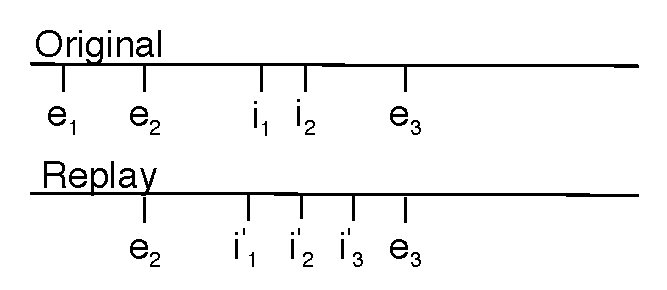
\includegraphics[width=\linewidth,height=0.8in]{../diagrams/state_machines/event_sequence.pdf}
%\end{wrapfigure}

In the general case it is always possible to construct two state machines that lead
to differing outcomes: one that only leads to the invariant violation when
we inject the next input
\emph{before} a new internal event, and another only when we inject \emph{after} a new internal
event. In other words, to be guaranteed to traverse any existing suffix that leads
to the invariant violation, we must recursively branch, trying both
possibilities for every new internal event. This implies an exponential number of
possibilities to be explored in the worst case.\footnote{
In our system~\cite{sts}, exponential search over these possibilities is not a practical option.
The heuristic our system uses when waiting for expected internal
events is to proceed normally if there are new internal events,
always injecting the next input when its last expected predecessor
either occurs or times out.}

\subsection{Modeling the Control Software}

If we assume a model of the control software's state machine, we can potentially
avoid exponential blowup. Assume we have a predicate $\Phi(\tau_P, a, b)$
that, given a prefix $\tau_P$ of events scheduled so far, and a pair of events $a$, $b$
(either external or internal), returns true whenever $\tau_P || a \rightarrow
b$ leads the software's state machine to a state $s$ s.t. some buggy state
$\hat{s}$ is reachable from $s$ along a sequence of labeled state transitions
$\alpha$, where the labels in $\alpha$
that correspond to external events are a subsequence of the remaining external inputs $E_S
\backslash \left\{ e \in \tau_P \right\}$. \colin{May want to remove the
requirement that $\alpha$ be a subsequence of external events.}
Here, a buggy state refers to
a state that produces a network configuration $c$ that violates a given
invariant.

For all prefixes $\tau_P || a\rightarrow b$ of $\tau_L$, if $\tau_L$ is a
superset of an MCS, then $\Phi(\tau_P, a, b)$ returns true.

For any new internal event $a$ and pending external event $b$, if
$\Phi(\tau_P, a, b)$ returns true, then we know that we can allow $a$ through
before $b$. In this way we can interleave new
internal events with our schedule of expected events $\tau_S$, and be
guaranteed to leave open the possibility of finding a divergent suffix through the
state machine that leads to an invariant violation.

\subsection{Obtaining a model}

Two ideas for obtaining $\Phi$: \\

\noindent{\bf Extrapolate from complete model.} There was a paper in
PLDI~\cite{vericon} where the authors
wrote their own controller and verified its entire state space. We could issue
queries on the state space to compute $\Phi$, and then extrapolate $\Phi$ for
other controllers assuming their state machines are sufficiently similar. \\

\noindent{\bf Infer partial models.} In general we want to
continue assuming that the control software is a black box.
Even with that constraint, we could infer a partial model of the control
software by observing its outputs across many executions, \ie~build a model
from logs. We might use Synoptic~\cite{beschastnikh2011leveraging} to compute
the model.


\section{Coping with Non-determinism}
\label{sec:non_determinism}
\documentclass{standalone}
\usepackage{multirow}
\usepackage{tabularx}
\usepackage{rotating}

\begin{document}

\begin{tabular}{| >{\centering\arraybackslash}p{1in} | >{\centering\arraybackslash}p{0.7in} | >{\centering\arraybackslash}p{1.15in} |}
\hline
{\bf Max replays per subsequence} & {\bf Size of final MCS} & {\bf Total hours}\\\hline\hline
1 & 65 & 6.10 \\\hline
2 & 20 & 6.37 \\\hline
3 & 15 & 7.78 \\\hline
4 & 12 & 9.59 \\\hline
5 & 9 & 6.38 \\\hline
6 & 9 & 11.20 \\\hline
7 & 9 & 11.83 \\\hline
8 & 6 & 12.35 \\\hline
9 & 6 & 11.13 \\\hline
10 & 6 & 12.86 \\\hline
\end{tabular}

\end{document}


\section{What Systems This Works Well On}
\label{sec:systems}
Two constraints: quiescence, and centralization.


\section{Partial Program Flow Analysis}
\label{sec:program_flow}
Suppose we ran program flow analysis on our mock network (to predict internal
events it will trigger), but not on the control software? This would still
allow us to remain agnostic to the language of the control software, but it might help us get better replay success.


% TODO: Include acknowledgements section
\renewcommand{\baselinestretch}{0.97}
\bibliographystyle{abbrv}
\bibliography{bib}


%\input{appendix}
%\theendnotes

\end{document}
